\documentclass{scrartcl}			% defines the kind of document you want to produce

% Include different packages:
\usepackage[utf8x]{inputenc}
\usepackage[T1]{fontenc}
\usepackage{lmodern}
\usepackage[english]{babel}
\usepackage{amsmath}
\usepackage{graphicx}           	% include graphics
\usepackage{caption}	
\usepackage{subcaption}	 
\usepackage{hyperref}
\usepackage{epstopdf}
\usepackage{siunitx}
\usepackage{float}

\title{Neuroprothetics Exercise 7\\Filter Banks}
\author{ Laura Bielenberg }
\date{28. Juni 2019}

\begin{document} 					% Document begins here

\maketitle

\section{A simplified cochlear implant model}
The code used to generate the following plots has been written using Python 3.7 and can be found under \texttt{code/exercise\_7.py} and \texttt{code/Neuroprosthetics/filter\_banks.py}.

\subsection{Border frequencies of a filter}\label{sec:borderfreq}
The band-pass filters in CIs range from about $\SI{100}{Hz}$ for the most apical electrode to $\SI{8}{kHz}$ for the most basal electrode. Using the \texttt{logspace()} function the border frequencies of the filters in a filterbank of CIs with 3, 6, 12 and 22 electrodes have been calculated as shown in figure~\ref{fig:border_freq}.
\begin{figure}[H]
\centering
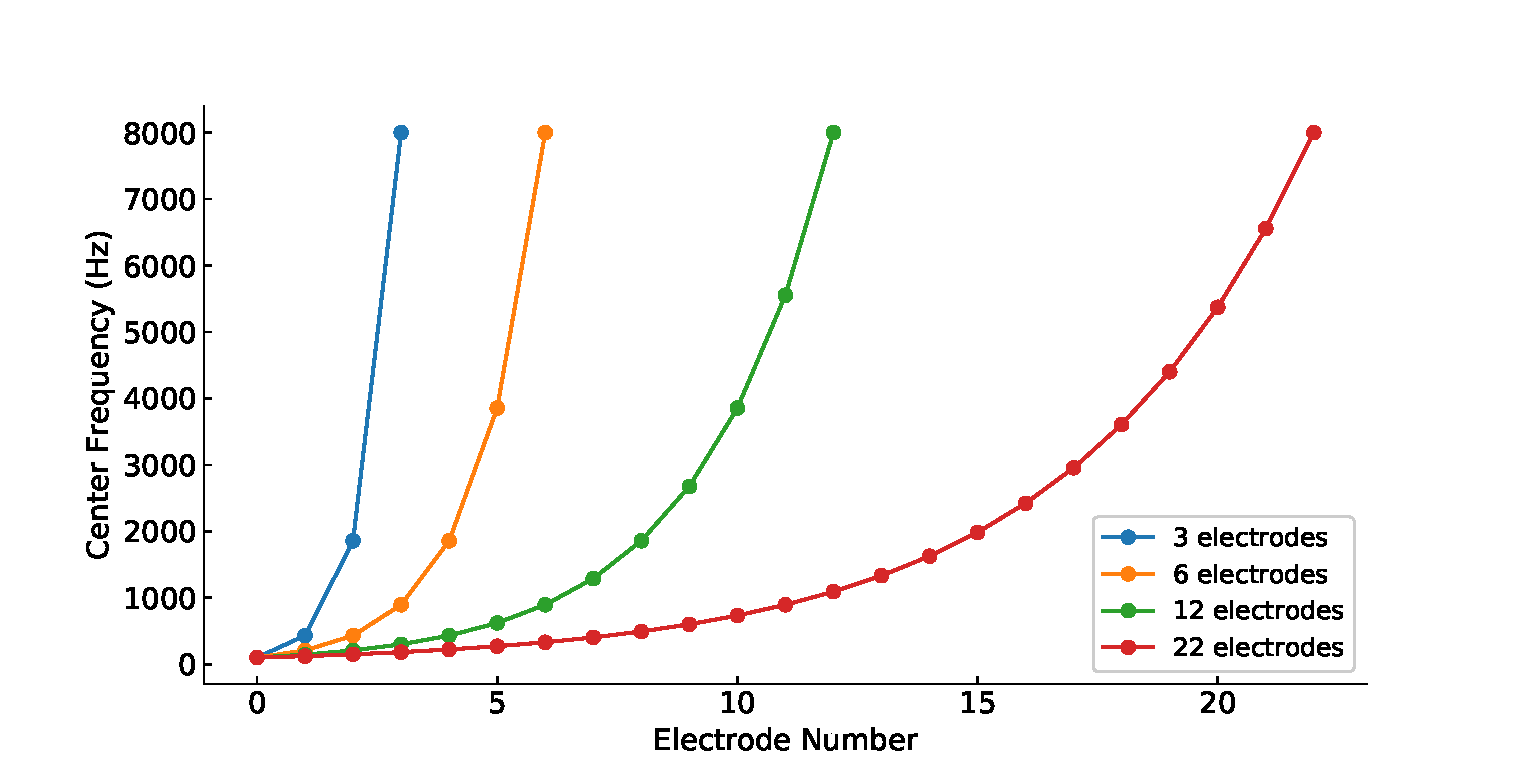
\includegraphics[width=0.9\linewidth]{imgs/center_frequencies_all.eps}
    \caption{Border frequencies for CIs with different numbers of electrodes and a frequency range of $\SI{100}{Hz}$ to $\SI{8}{kHz}$ } 
    \label{fig:border_freq} 
\end{figure}

\subsection{Implement a filter bank}
The task was to implement a second-order band-pass filter bank with the border frequencies from section~\ref{sec:borderfreq} for all given CI types using a butterworth filter. 

\subsubsection{Filterbank responses}
For the band-pass filter implementation I used the \texttt{butter()} function provided by the Python \texttt{scipy.signal} library.
Figure~\ref{fig:freq_resp} shows the the frequency response of the filter bank for CIs with 3 and 22 electrodes on a double-logarithmic scale. It can be seen that in both cases the response curves of two neighbouring filters cross at their  $\SI{-3}{dB}$ point.

\begin{figure}[H]
  \begin{subfigure}[b]{\linewidth}
    \centering
	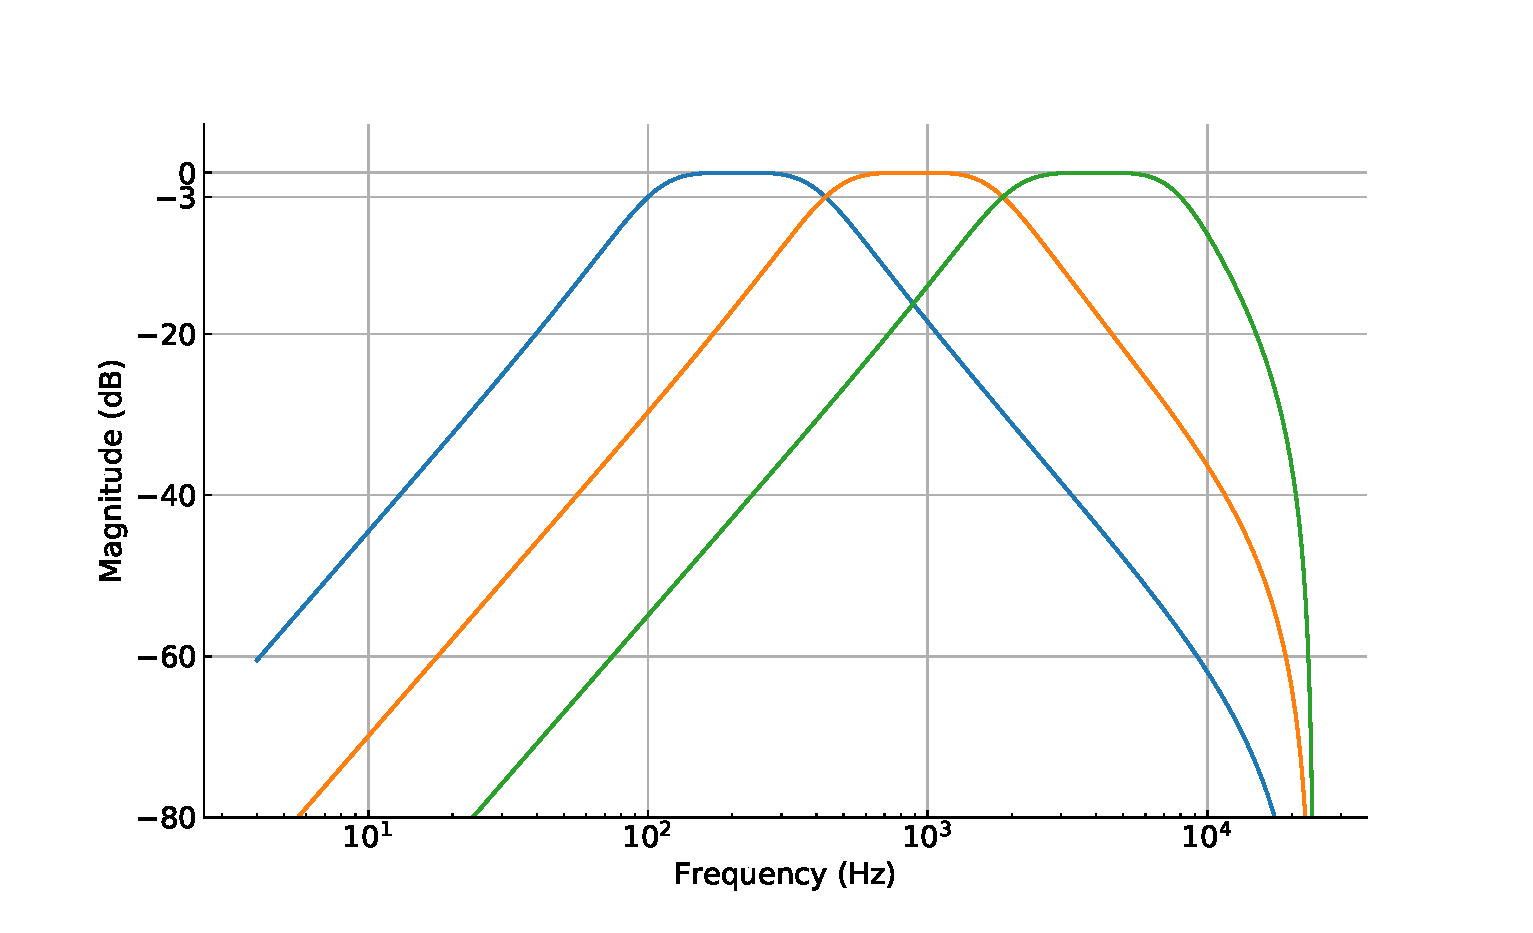
\includegraphics[width=0.9\linewidth]{imgs/ci_with_3_electrodes.eps}
    \caption{requency response for a CI with three electrodes.} 
    \label{fig:ci_3} 
    \end{subfigure}
    \quad
      \begin{subfigure}[b]{\linewidth}
   	 \centering
   	 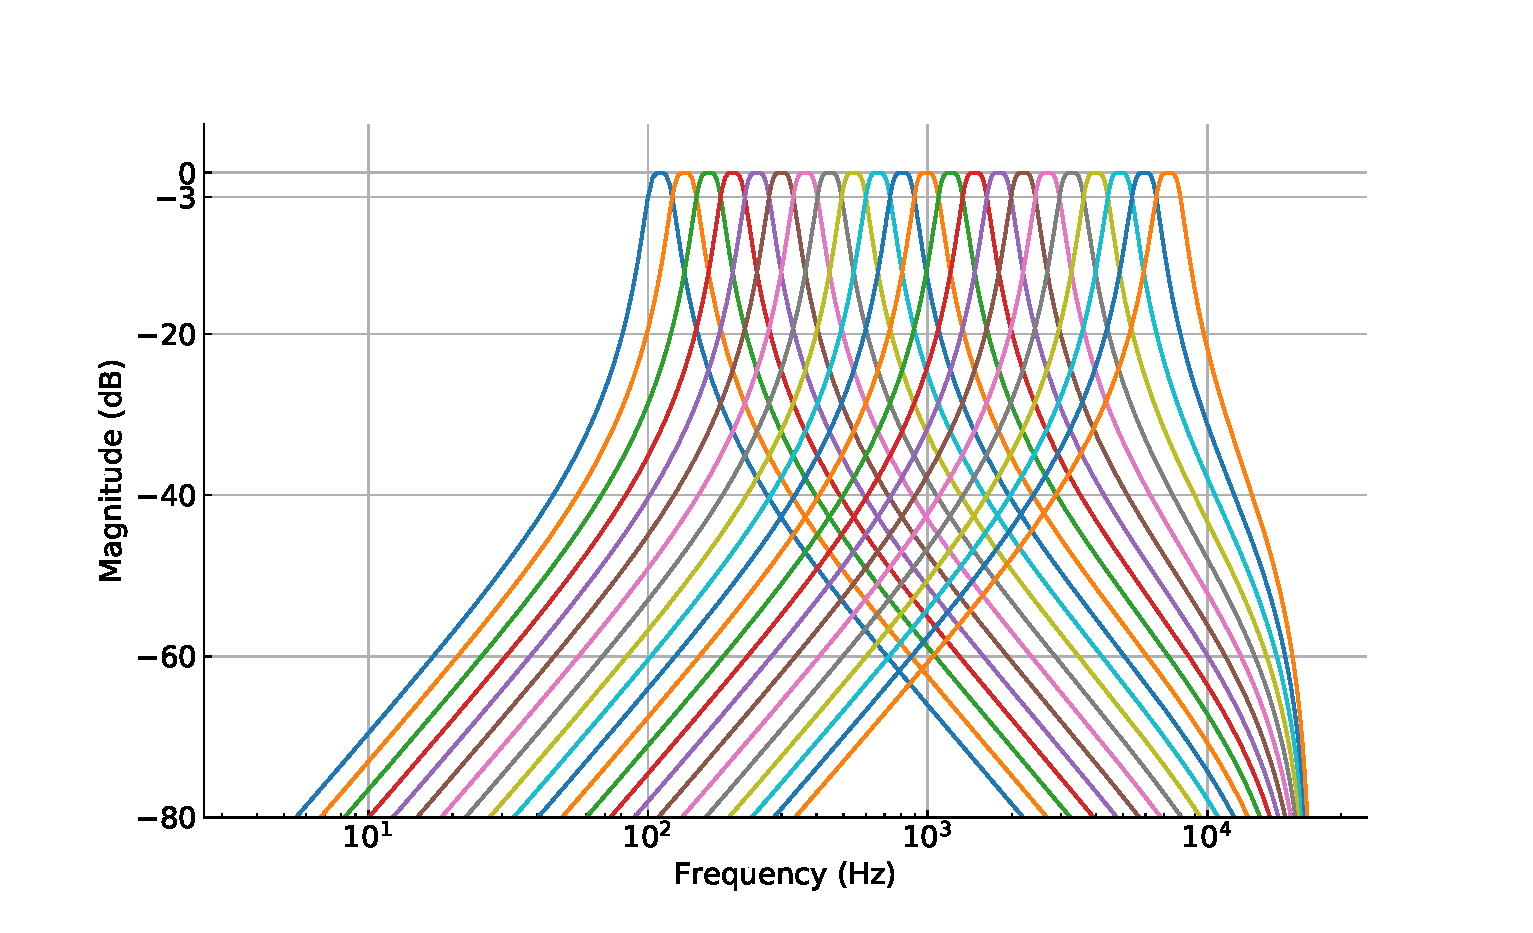
\includegraphics[width=0.9\linewidth]{imgs/ci_with_22_electrodes.eps}
    \caption{Frequency response for a CI with 22 electrodes.} 
    \label{fig:ci_22} 
    \end{subfigure}
    \caption{Frequency response of a second-order  band-pass filter bank for different CI types.}
    \label{fig:freq_resp}
\end{figure}

\newpage
\subsubsection{Filter a recorded signal}
It was asked to record an acoustically interesting word which should be more than a second long, and include both plosives (e.g.\textit{’k’}) and fricatives (e.g\textit{’s’})) with a microphone. I chose the word \textit{Sorekara} (jap.: and then) for this and recorded it with a sampling rate of $f_s = \SI{44.1}{kHz} $. Figure~\ref{fig:sore} shows the original, unfiltered audio signal.\\
It was then filtered with the filter banks. The time signal of each filter channel of a 12-electrode CI can be seen in figure~\ref{fig:sore_22}.  Furthermore, Figures~\ref{fig:sore_fft} and \ref{fig:sore_22_fft} show the normalised frequency response of the original signal and for each filter channel of a 12-electrode CI.\\The first three to four filters make it very difficult to understand the spoken word at all. In the middle ones, aprox. filters five to  seven, the 's' and 'k' sound is the clearest, while in the remaining filtered sounds of filter eight to 12, the 's' sound is the most intense one. 

\begin{figure}[H]
\centering
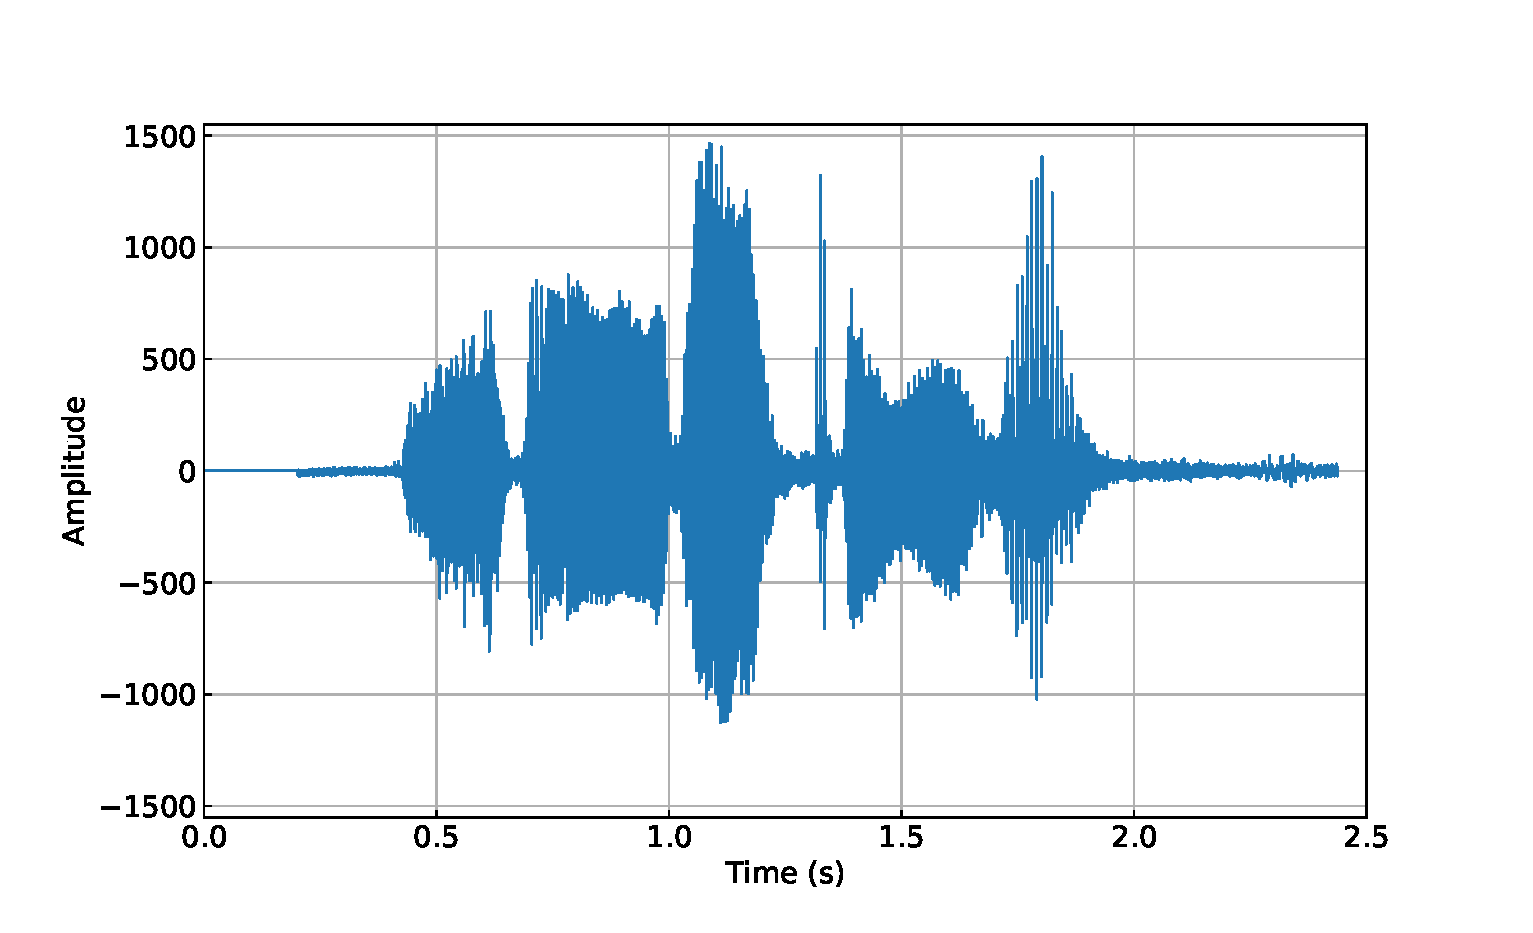
\includegraphics[width=0.8\linewidth]{imgs/sorekara.eps}
    \caption{Time signal of the recorded sound.} 
    \label{fig:sore} 
\end{figure}

\begin{figure}[H]
\centering
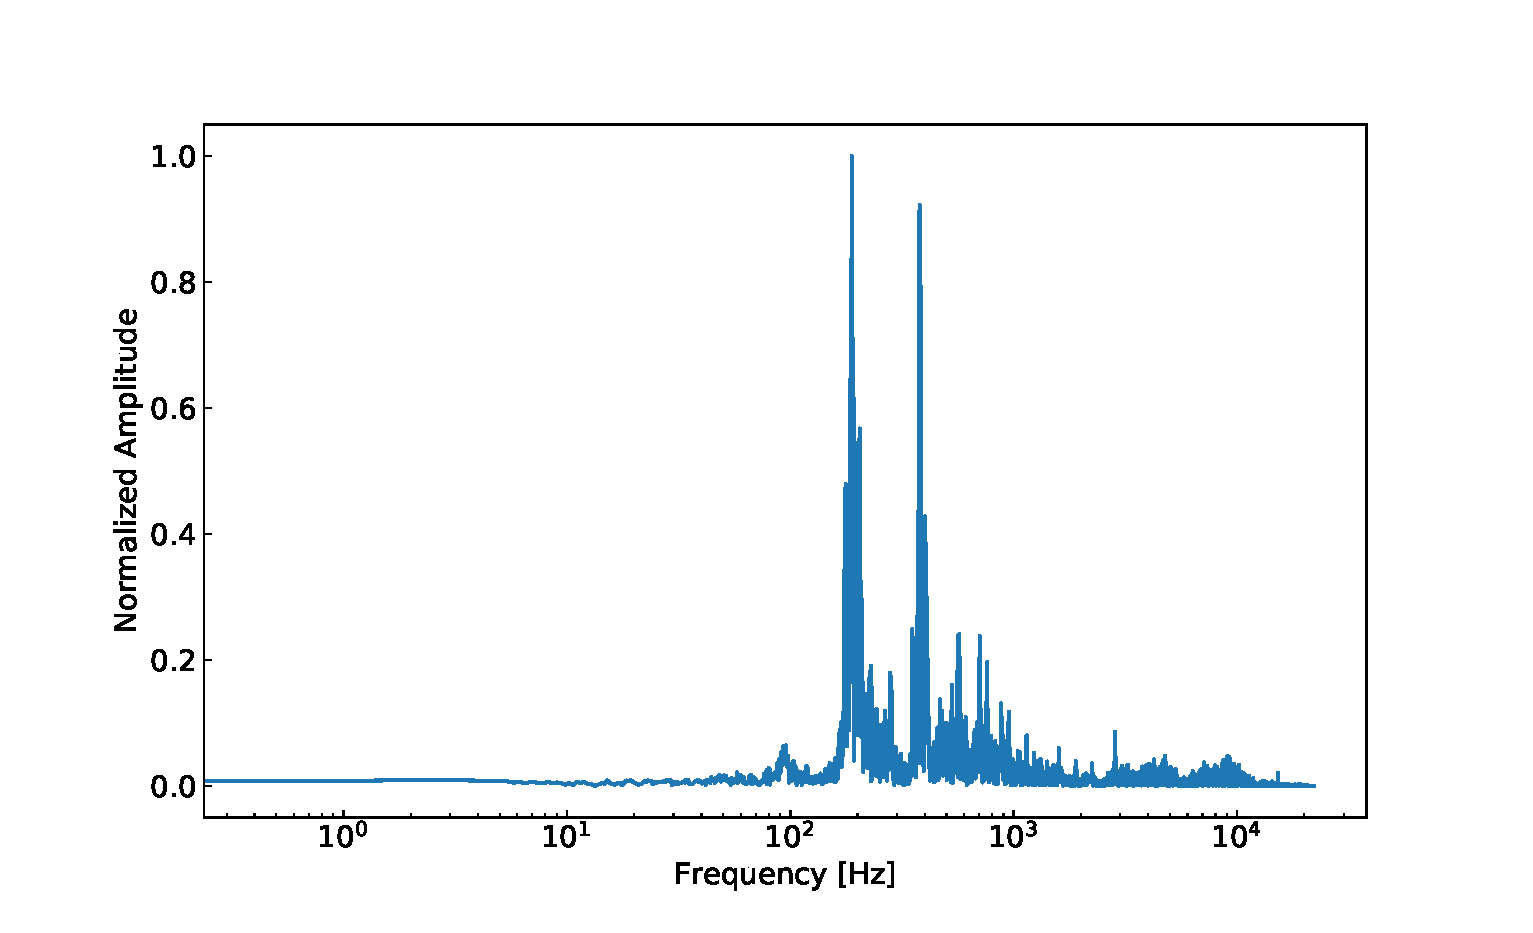
\includegraphics[width=0.8\linewidth]{imgs/sorekara_fft.eps}
    \caption{Frequency response of the recorded sound.} 
    \label{fig:sore_fft} 
\end{figure}

\begin{figure}[H]
\centering
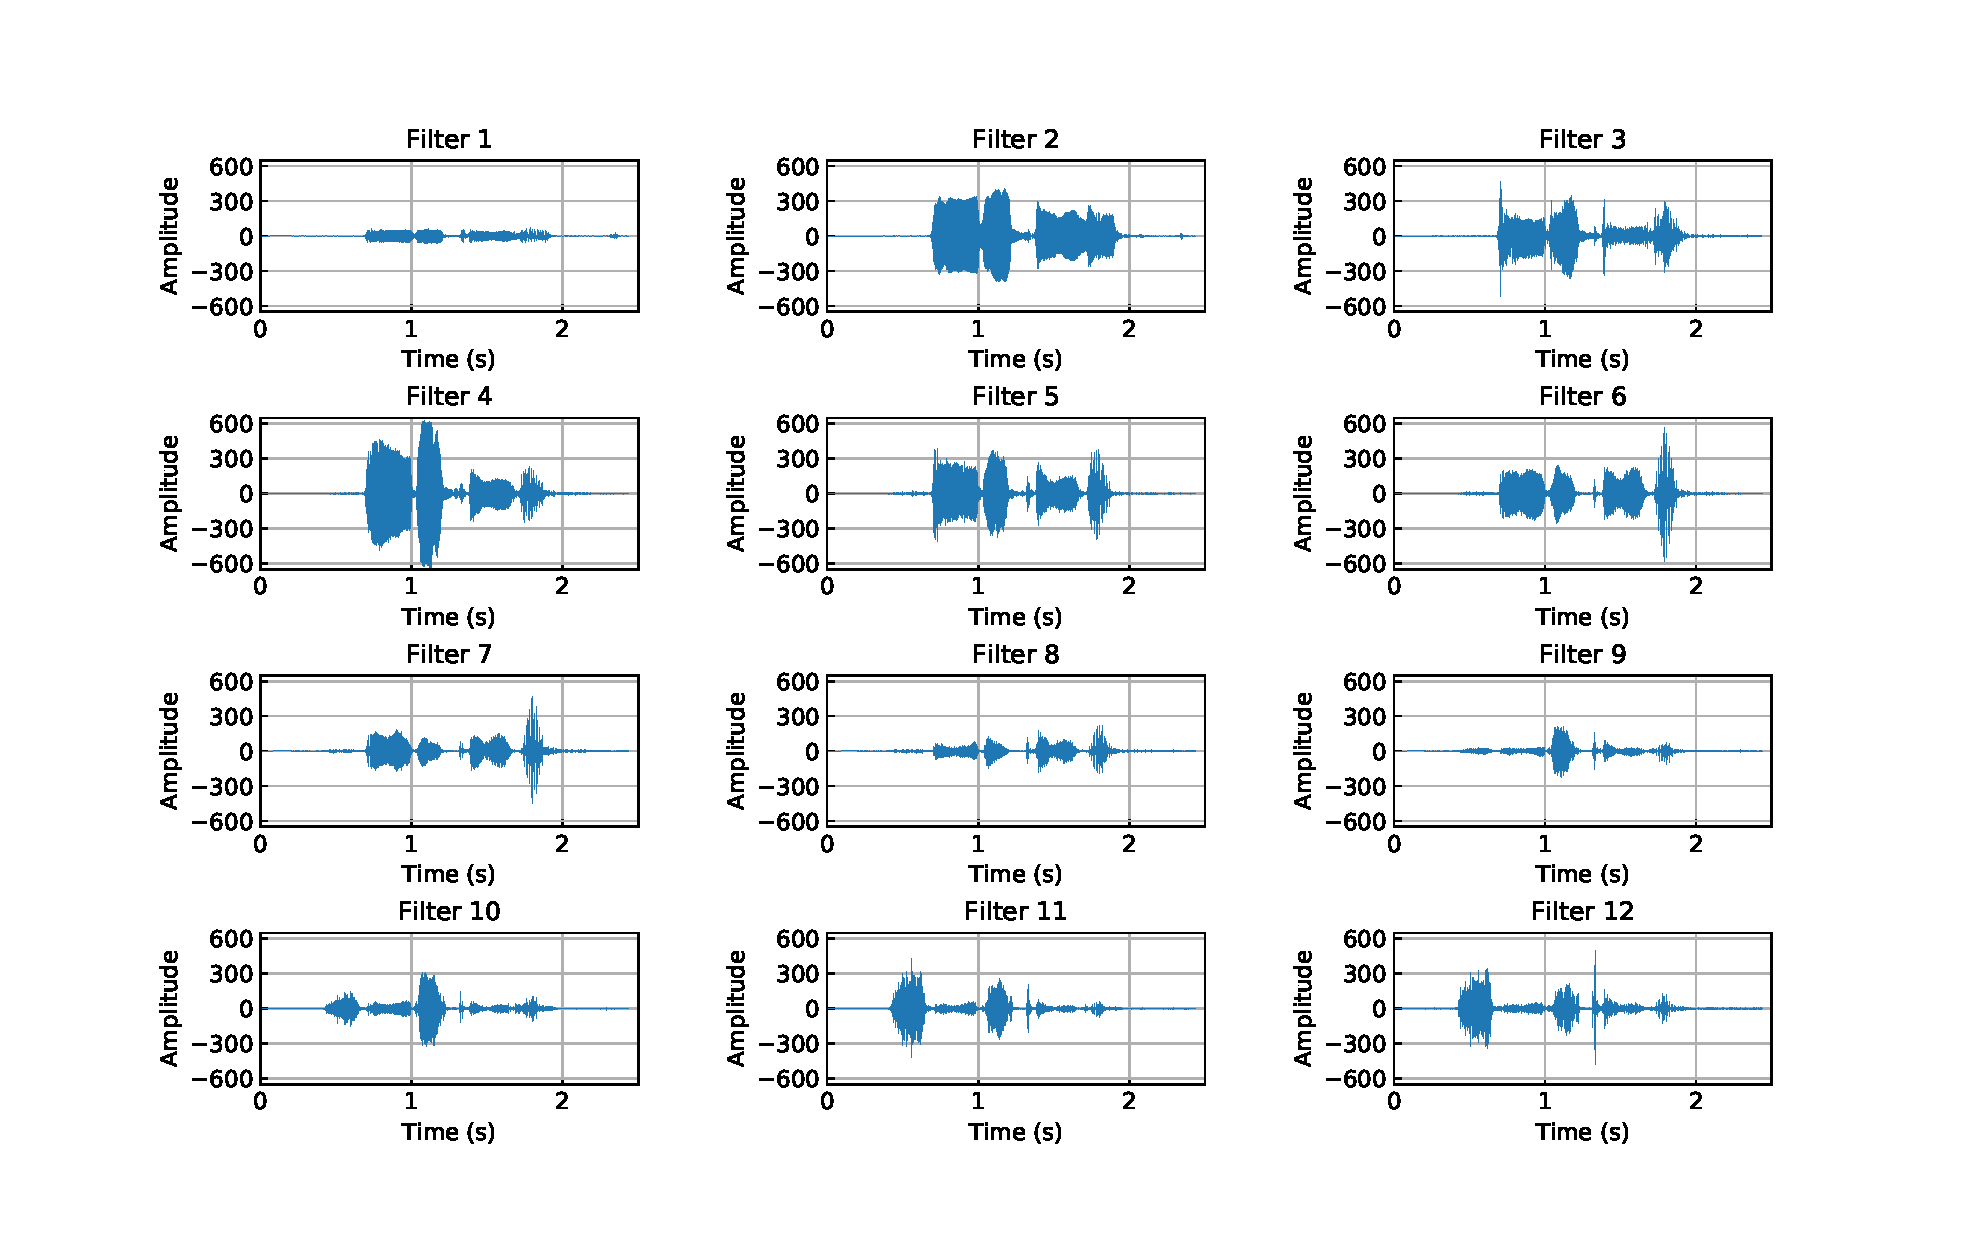
\includegraphics[width=\linewidth]{imgs/wav_results.eps}
    \caption{Time signals of the filtered sounds for each channel of a 12 electrode CI.} 
    \label{fig:sore_22} 
\end{figure}

\begin{figure}[H]
\centering
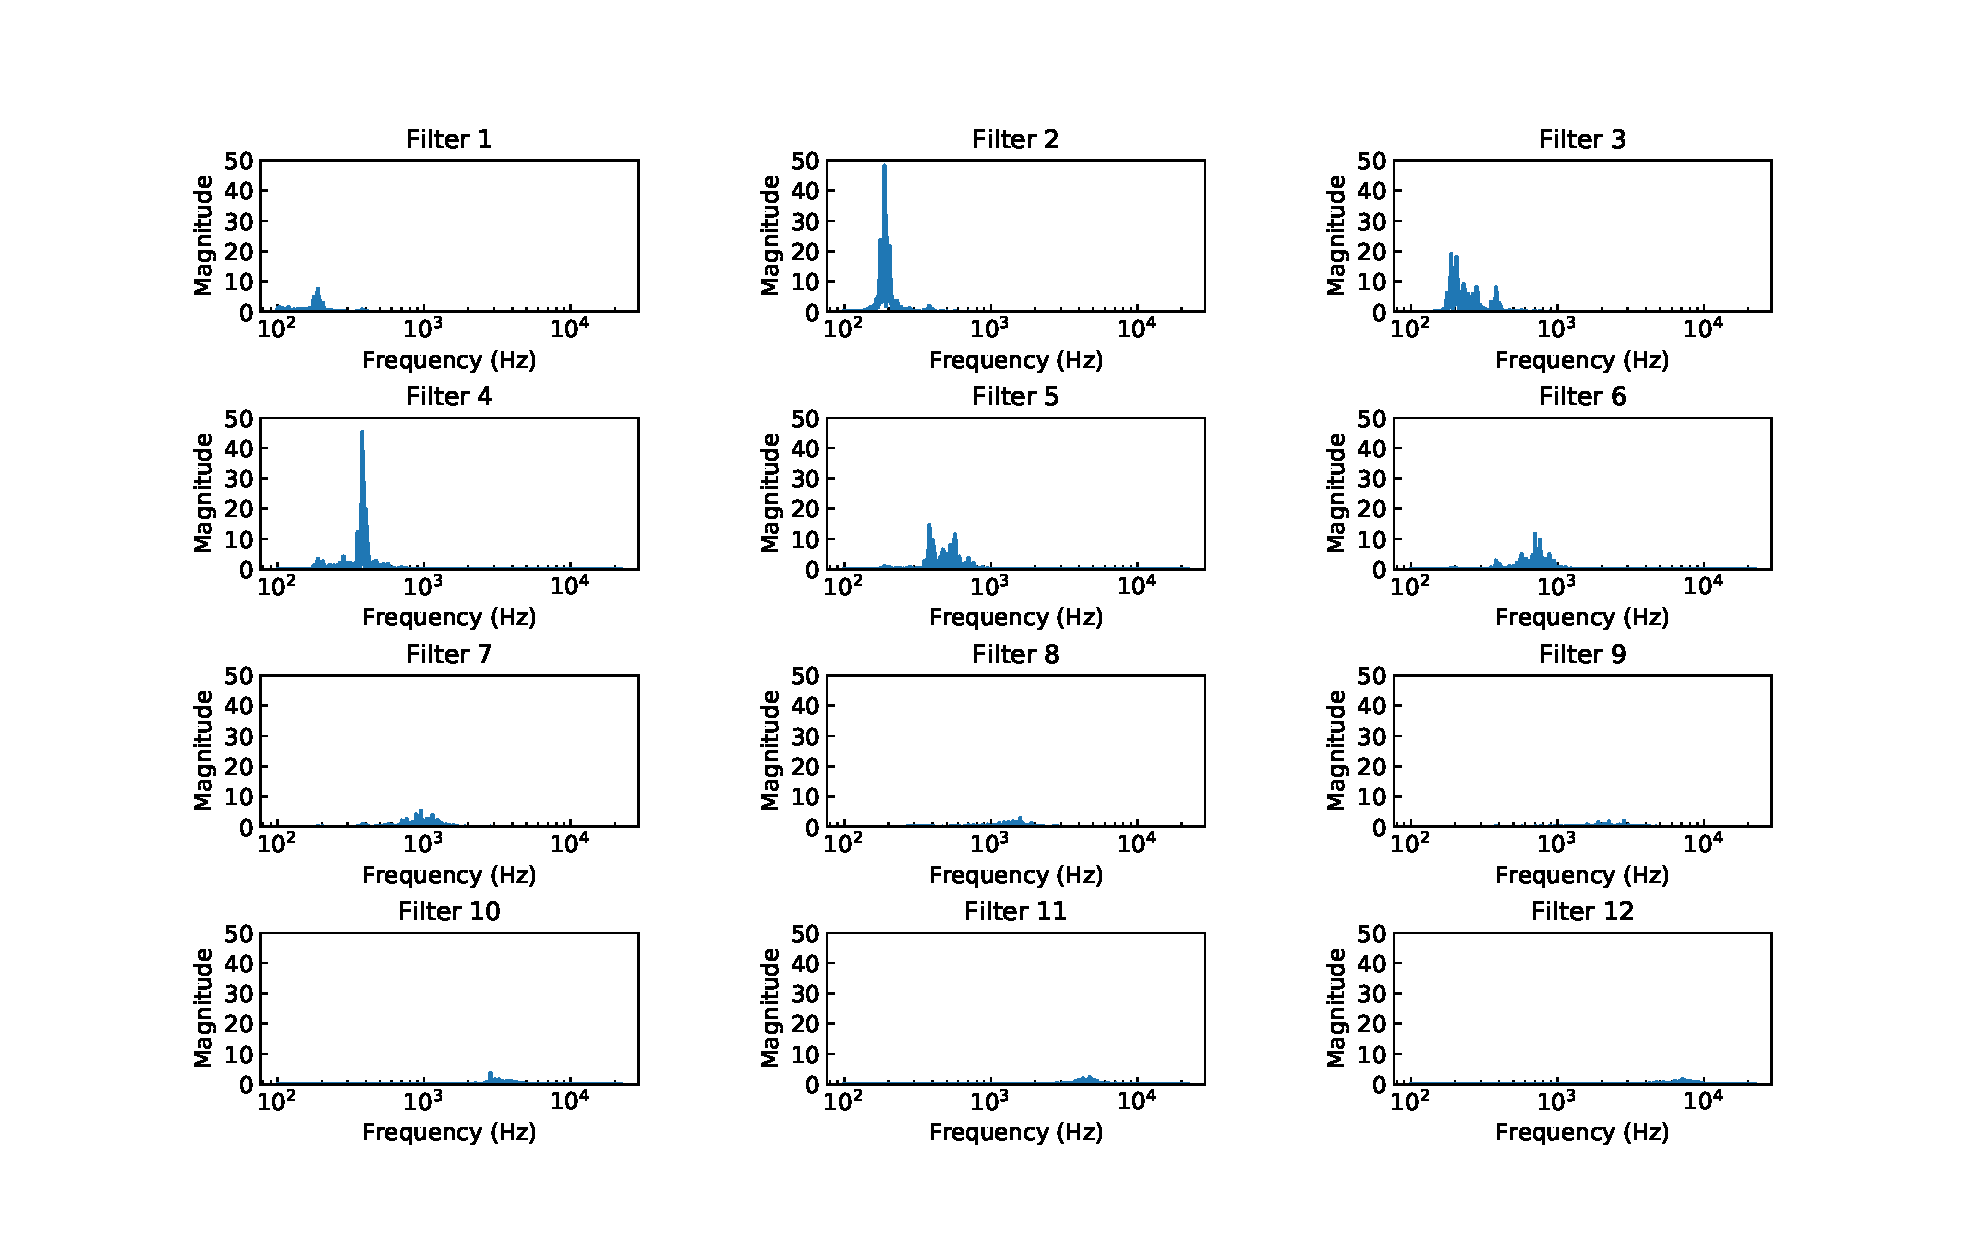
\includegraphics[width=\linewidth]{imgs/wav_results_fft.eps}
    \caption{Frequency responses of the filtered sounds for each channel of a 12 electrode CI.} 
    \label{fig:sore_22_fft} 
\end{figure}

\subsection{Join the channals}
The charactiristic of a band-pass filter is, that it hardly affects the signal within its bandwidth, but damps the signal outside of the band-pass region. Since each of the filters used in this experiment causes an amplitude decrease of $\SI{-3}{dB}$ at its band-pass border frequencies, the summed signals will show corresponding frequency gaps, at which the signal amplitude is decreased accordingly. Because of that, those parts of the signal which lie in one of the frequency gaps and which have a comparably low amplitude with respect to the signal in the neighbouring filter bands, will be suppressed in the resulting sum signal.\\Listening to the resulting signals, the summed 3 electrode CI sounds the worst, as it damps a lot of the signal in the 115 - 120 Hz range, where one of two frequency peaks of the signal is situated. The 6, 12 and 22 electrode CIs on the other hand sound rather similar to eachother.\\ This can also be seen in the spectograms, where figure~\ref{fig:spec_ci_3} shows only a little band of active frequencies, while the other spectogram plots show broughter ranges. All of the spectograms show medium magnitudes (blue/green) for the first sillable 'so', high magnitudes (red) in the middle of the spoken word around where the sillable 're' is being said, and low magnitudes for the last two sillables 'ka' and 'ra'.
\begin{figure}[H]
\centering
	 \begin{subfigure}[b]{0.49\linewidth}
    		\includegraphics[width=\linewidth]{imgs/spectogram_3_CI.eps}
   		 \subcaption{Spectogram for a three electrode CI.} 
   		 \label{fig:spec_ci_3} 
   		 \end{subfigure}
   		 \begin{subfigure}[b]{0.49\linewidth}
    		\includegraphics[width=\linewidth]{imgs/spectogram_6_CI.eps}
   		 \subcaption{Spectogram for a six electrode CI.} 
   		 \label{fig:spec_ci_6} 
   		 \end{subfigure}
   		 \begin{subfigure}[b]{0.49\linewidth}
   		 \includegraphics[width=\linewidth]{imgs/spectogram_12_CI.eps}
   		 \caption{Spectogram for a 12 electrode CI.} 
   		 \label{fig:spec_ci_12} 
   		 \end{subfigure}
   		 \begin{subfigure}[b]{0.49\linewidth}
   		 \includegraphics[width=\linewidth]{imgs/spectogram_22_CI.eps}
   		 \caption{Spectogram for a 22 electrode CI.} 
   		 \label{fig:spec_ci_22} 
   		 \end{subfigure}
   		\caption{Spectograms of the sum-signal for different CI types}
   		\label{fig:spectograms}
\end{figure}

\begin{figure}[H]
\centering
	 \begin{subfigure}[b]{0.49\linewidth}
    		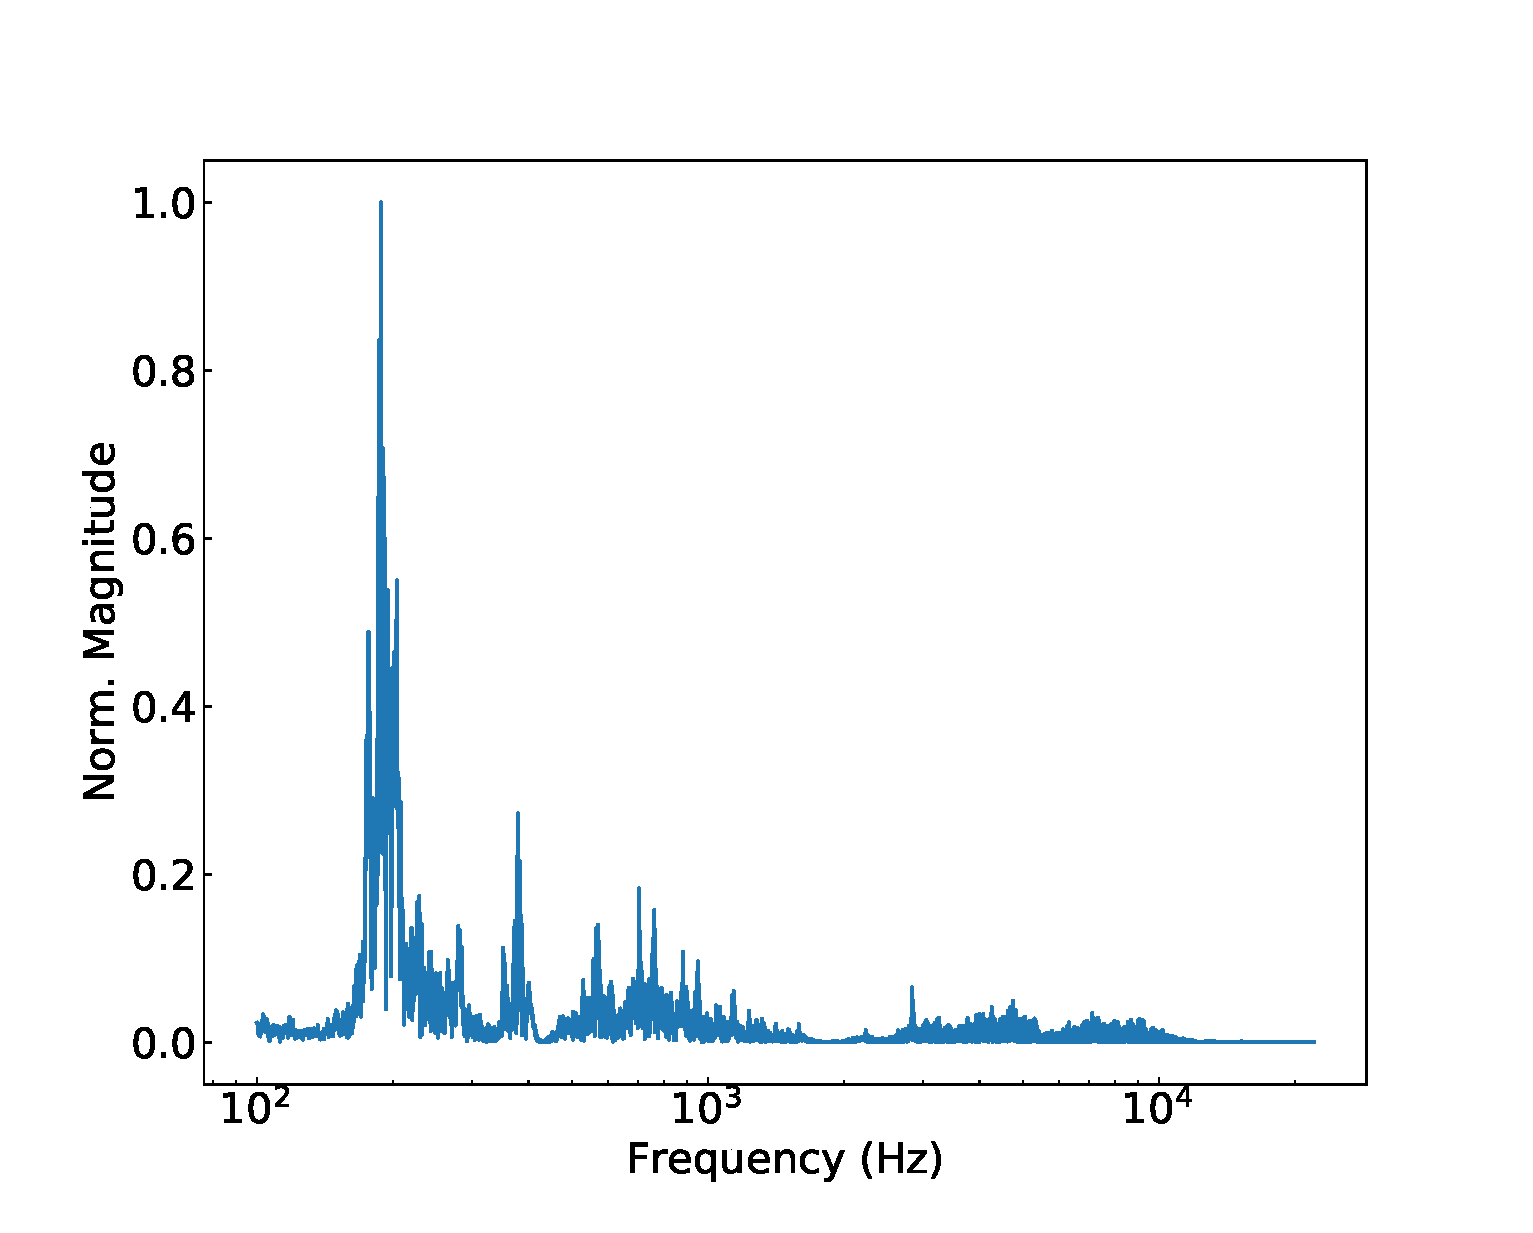
\includegraphics[width=\linewidth]{imgs/filtered_3_fft.eps}
   		 \subcaption{Spectrum for a three electrode CI.} 
   		 \label{fig:ci_3} 
   		 \end{subfigure}
   		 \begin{subfigure}[b]{0.49\linewidth}
    		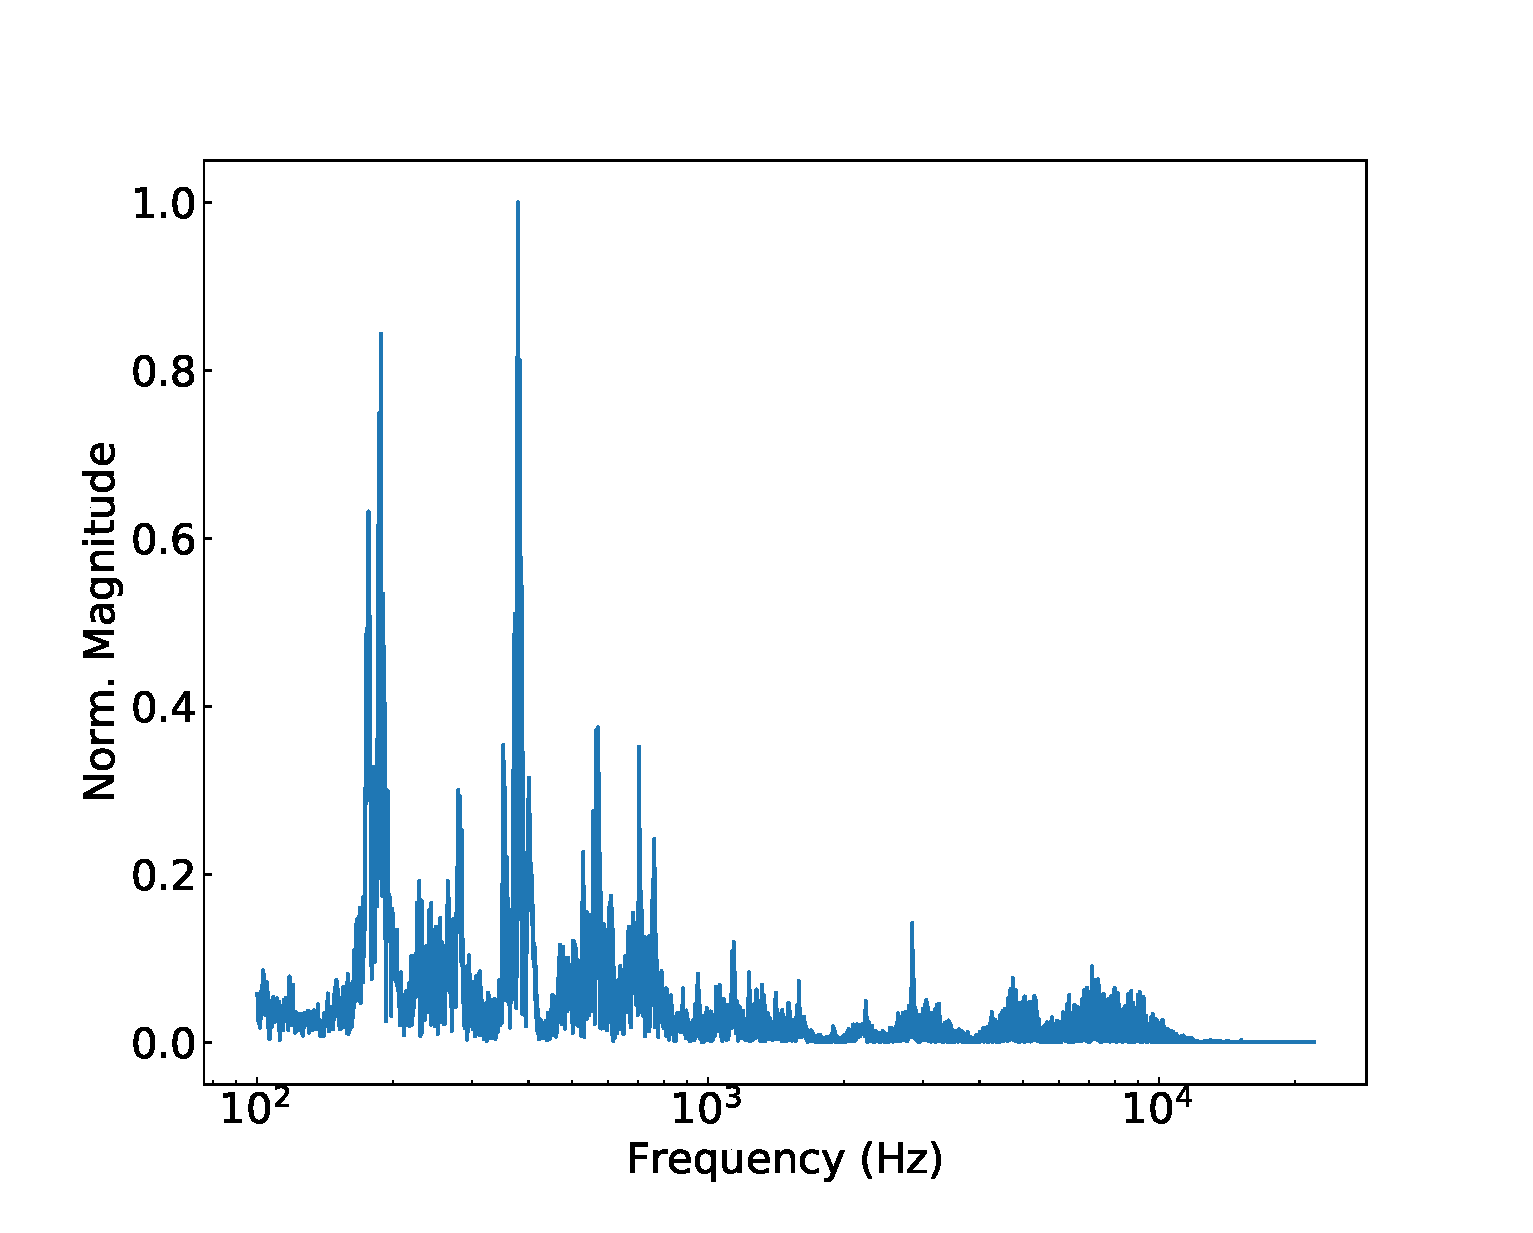
\includegraphics[width=\linewidth]{imgs/filtered_6_fft.eps}
   		 \subcaption{Spectrum for a six electrode CI.} 
   		 \label{fig:ci_3} 
   		 \end{subfigure}
   		 \begin{subfigure}[b]{0.49\linewidth}
   		 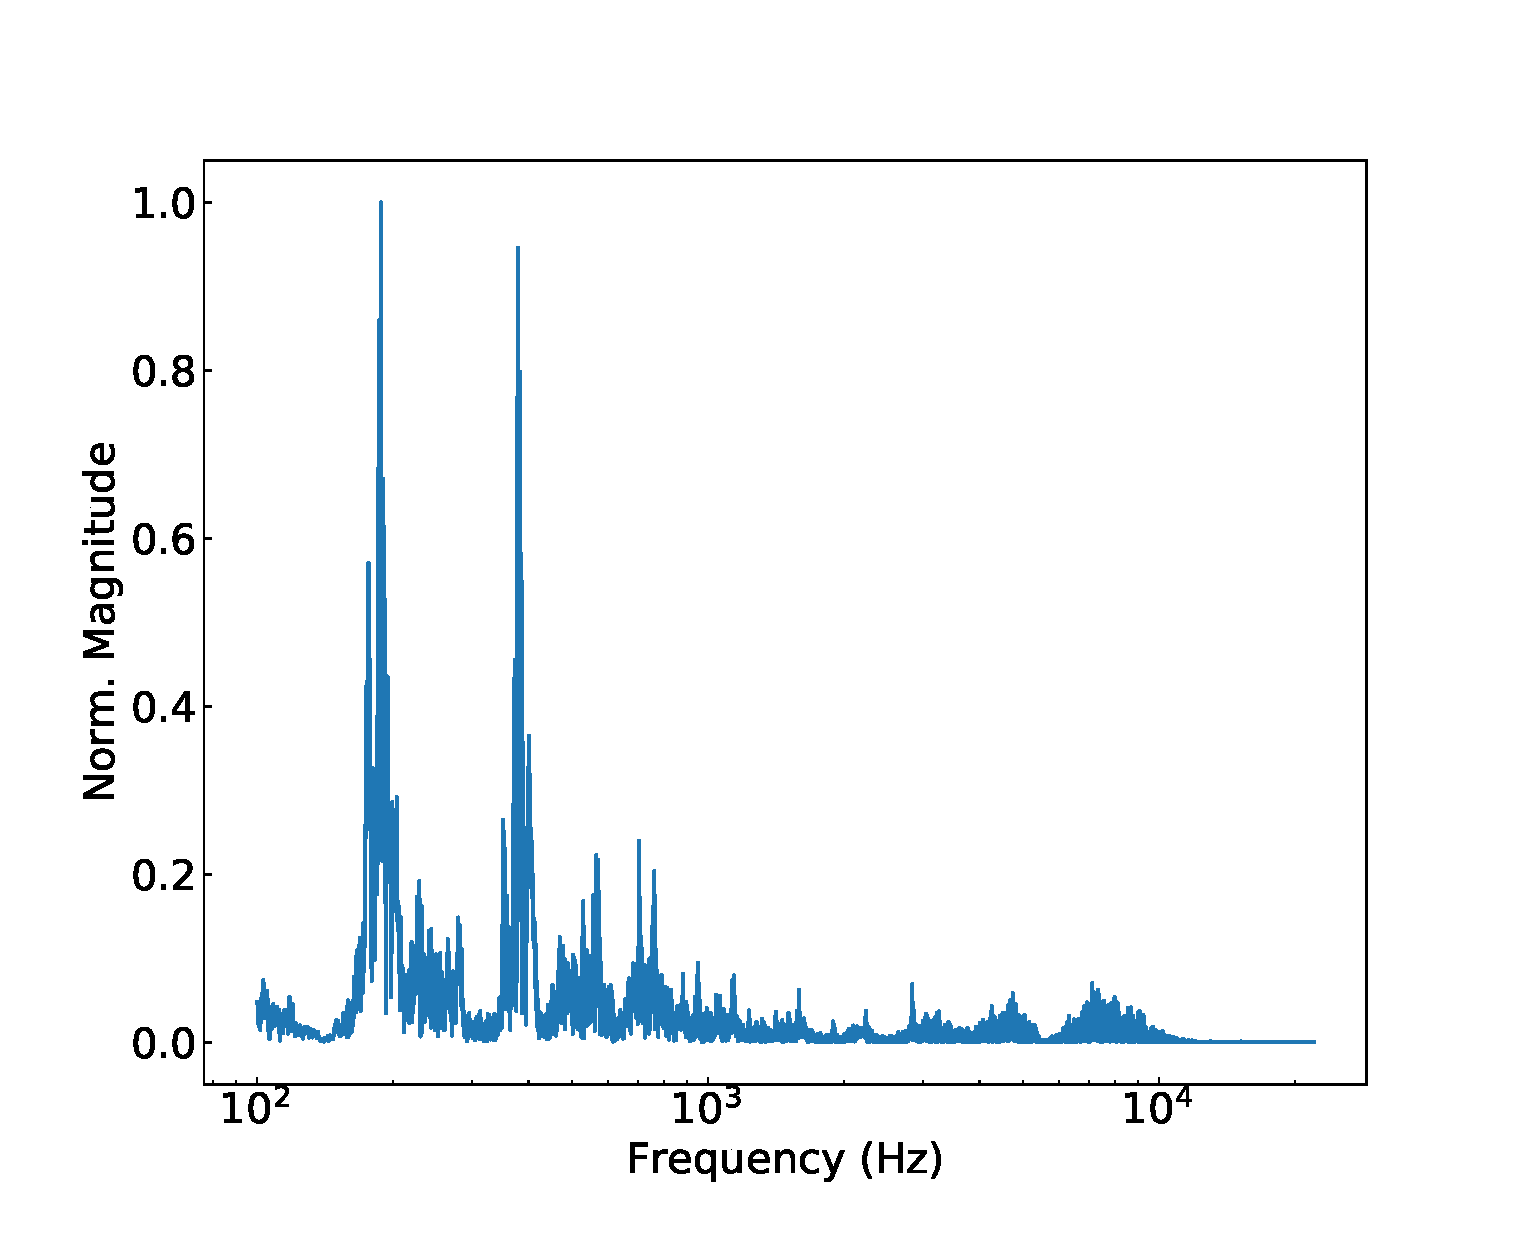
\includegraphics[width=\linewidth]{imgs/filtered_12_fft.eps}
   		 \caption{Spectrum for a 12 electrode CI.} 
   		 \label{fig:ci_3} 
   		 \end{subfigure}
   		 \begin{subfigure}[b]{0.49\linewidth}
   		 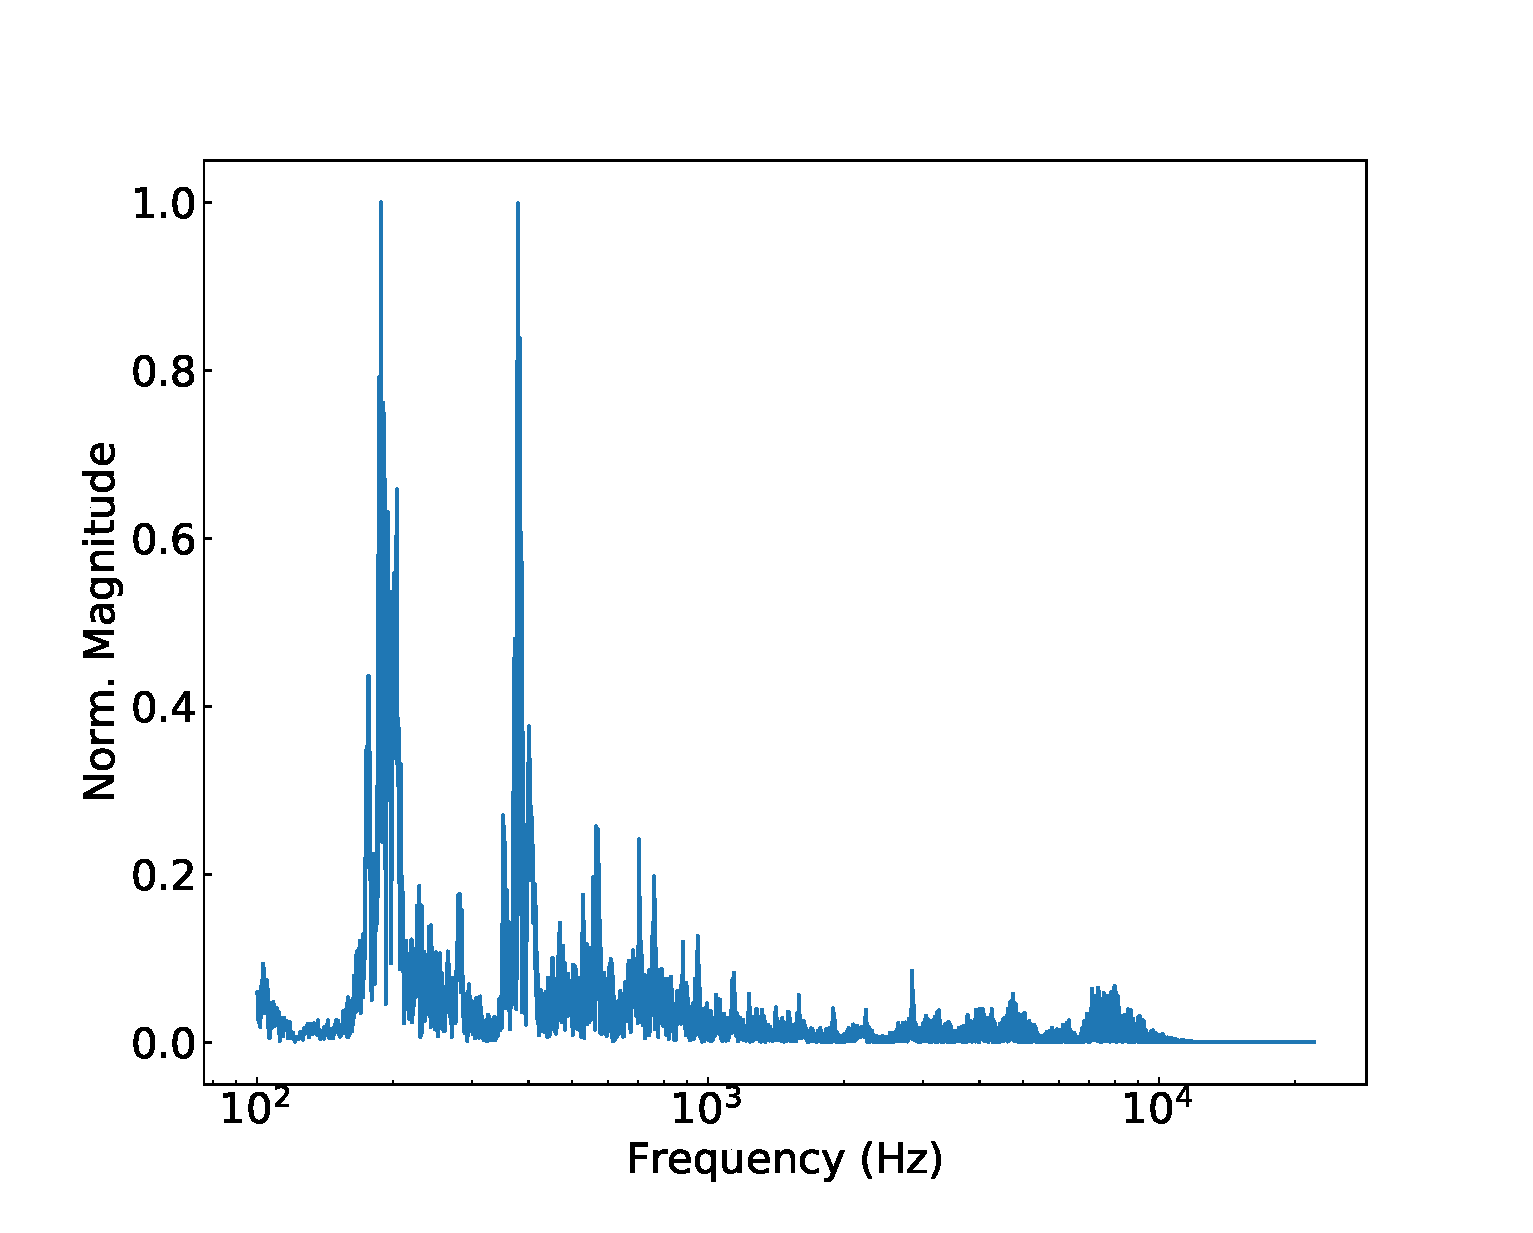
\includegraphics[width=\linewidth]{imgs/filtered_22_fft.eps}
   		 \caption{Spectrum for a 22 electrode CI.} 
   		 \label{fig:ci_3} 
   		 \end{subfigure}
   		\caption{Frequency spectrum of the sum-signal for different CI types}
   		\label{fig:spectograms}
\end{figure}

\end{document}
